%% mapping.tex

\section{Geometry mapping and associated tools}

\pn  In the  previous section,  we have  presented the  basic concepts
(GID,  hierarchy rules,  GID manager)  used in  the \texttt{geomtools}
library.  Now it is time to introduce some high-level functionnalities
that  can  be  implemented  on  top  of  these  low-level  concepts  :
\emph{geometry mapping} and \emph{locators}.

\subsection{Geometry mapping}

The key  concept of \emph{geometry mapping}  is to allow  the users to
benefit of some automated (or semi-automated) database of all (or part
of) the objects that belongs  to a geometry hierarchical setup. Such a
database will naturally  use the object's GID as  the primary keys for
accessing some meta-data associated to an object.

As seen  in the previous sections,  it is possible to  define some non
ambiguous  \emph{hierarchy  rules}   to  reflect  the  mother/daughter
relationships between objects  of a virtual geometry setup.  This is a
task  for  the   GID  manager  object,  which  is   available  in  the
library. 

However,  when designing the  numbering scheme,  there are  still many
arbitrary choices that have to  be made by the architect/developper of
the numbering  scheme built  on top  of the geometry  model :  ''Do we
start the  values of subaddresses  from \texttt{0} or  \texttt{1} when
several  replicates of  some category  are  placed in  a given  mother
volume ?'', ''What value is chosen for the subaddress of the left part
of  this tracking  chamber :  O or  1 ?'',  ''What integer  values are
associated to the North, South, West and East directions ?''\dots \ So
we  need  some  additional  conventions  and  rules  to  finalize  the
addressing scheme.  Then we  will be able  to establish and  build the
full list of GIDs that makes sense in our application.

If  we  consider the  above  \emph{domestic}  virtual  world, we  have
implicitely used such rules on top of the hierarchy rules. We now need
some tools to automatically inform  the geometry model of these rules.
Let's  build  such  a  virtual   setup  with  the  tools  provided  by
\texttt{geomtools}. Then  we will  see how to  enrich this  model with
special \emph{mapping directives}.

 

\subsection{Mapping directives}

Mapping directives explains the  rules and conventions to be respected
by  dedicated  algorithms  that  are  responsible  for  the  automatic
generation of  GIDs associated to  the physical volumes of  a geometry
hierarchy.   These   algorithms  first  need  a   GID  manager  object
(\texttt{geomtools::id\_mgr} class) in order to know the layout of the
numbering scheme to be applied to the geometry hierarchy.  On a second
step, mapping directives  are used to build the  GID associated to all
physical volumes requested  by users and associate each  GID with some
specific informations.

The  \texttt{geomtools::mapping} class  implement  such an  algorithm.
Given  a   \emph{model  factory}   and  a  \emph{GID   manager},  this
\emph{mapping algorithm} establishes a  list of all requested GIDs and
associates them with some useful geometry informations :

\begin{itemize}

\item  the placement (position  and rotation  matrix) of  the physical
  object in the \emph{world} volume;

\item a reference to the \emph{logical volume} it refers to,

\item a list of auxiliary properties.

\end{itemize}
This results  in the  creation of a  -- possibly large  -- dictionnary
that  contains the  geometry information  requested for  some physical
volumes.  The  GID of  a given volume  is used  as the primary  key to
access the informations from this \texttt{GID database}.


Practically,  the \texttt{geomtools}  library proposes  to  enrich the
description  of the  geometry models  that take  part to  the geometry
setup  by   adding  some  additionnal  properties   dedicated  to  the
\emph{mapping} functionnality.

From the  \emph{geometry modelling tutorial}  we have learnt  to write
the description of a \emph{geometry model}.  In the following example,
we  recognize  a few  configuration  directives  for a  \emph{stacked}
geometry model  : material, length  unit, description of  the geometry
models to  be stacked  along some axis  (properties starting  with the
\TT{stacked.}  prefix).   We also recognize  visualization directives,
starting with the \TT{visibility.}  prefix :

\begin{ShellVerbatim}
[name="stacked_box" type="geomtools::stacked_model"]
material.ref            : string  = "__default__"
length_unit             : string  = "cm"
stacked.axis            : string  = "z"
stacked.number_of_items : integer = 4
stacked.model_0         : string  = "blue_cylinder"
stacked.label_0         : string  = "stacked_0"
stacked.model_1         : string  = "huge_red_box"
stacked.label_1         : string  = "stacked_1"
...
visibility.hidden       : boolean   = 0
visibility.color        : string    = "grey"
...
\end{ShellVerbatim}

The  \emph{mapping}  directives  will   use  a  similar  grammar.   By
convention, they will start with the \TT{mapping.} prefix. We will see
below what is  the syntax for these directives.   But first let's come
back to some concept we have explored so far.

We have  shown previously  that the GID  attached to  a \emph{physical
  volume} is not an intrinsic property of the associated \emph{logical
  volume} from  which the physical  volume is built/modelled  and thus
not a  property of the corresponding \emph{geometry  model}. The point
here is that it is the action to place a logical volume in some mother
volume that  \emph{instantiates} the physical volume. The  GID is thus
instantiated too at  this step.  It means that  the description of the
mother volume  should contain the mapping directives  for its daughter
volumes.

Practically,  there  is only  one  useful  mapping  directive that  is
implemented  in \texttt{geomtools},  namely \TT{mapping.daughter\_id}.
It is used in a parameterized  way, i.e. is must be appended with some
special string label (with an additionnal dot character):
\begin{verbatim}
mapping.daughter_id.<XXXXX> : string = "<MAPPING DIRECTIVE>"
\end{verbatim}
\pn where :

\begin{itemize}

\item \texttt{<XXXXX>} is a  label that identifies non-ambiguously one
  of  the daughter volumes  contained in  the current  geometry model,
  i.e. the \emph{mother},

\item \texttt{<MAPPING  DIRECTIVE>} is  a character string  that gives
  the rules to build the GID associated to this daughter volume.
  
  The allowed syntaxes for \texttt{<MAPPING DIRECTIVE>} are:
  \begin{itemize}
  \item for volumes belonging to some \emph{inherited} geometry categories :
    \begin{center}
      \texttt{[<CATEGORY NAME>]}
    \end{center}
  \item for volumes belonging to some \emph{extended} geometry categories :
    \begin{center}
      \texttt{[<CATEGORY NAME>:<SUBADDRESS NAME 1><OP 1><SUBADDRESS VALUE 1>(,<SUBADDRESS NAME 2><OP 2><SUBADDRESS VALUE 2>)]}
    \end{center}
  \end{itemize}
  \pn where :
  \begin{itemize}
    
  \item 
    \texttt{<CATEGORY NAME>} is the  name of a geometry category known
    by the \emph{GID manager}
    
  \item
    \texttt{<SUBADDRESS NAME 1>}  is the name of a  subaddress that is
    part  of the  addresses path  description known  by  the \emph{GID
      manager}

  \item
    \texttt{<OP 1>} is the \verb+=+ ot the \verb-+- operator,

  \item
    \texttt{<SUBADDRESS VALUE 1>} is an integer value (>=0)

  \item  the\texttt{(,<...>)}  indicates  that  the  numbering  scheme
    accept more similar rules.
  \end{itemize}


\end{itemize}

\pn Examples in the context of the domestic virtual setup :
\begin{itemize}

\item \texttt{[house:house\_number=666]} : an object in the \TT{house}
  category of which the \TT{house\_number} is set explicitely at value
  \texttt{666},

\item \texttt{[floor:floor\_number+0]}  : an object  in the \TT{floor}
  category  of which  the \TT{floor\_number}  is  autoincremented from
  starting value \texttt{0}; the  \texttt{house\_number} of the GID is
  supposed  to be  automatically set  because the  \TT{floor} category
  extends the \TT{house} so the GID  of this floor object will use the
  \texttt{house\_number} of the mother house.

\item  \texttt{[jewel:row\_number=0,column\_number=1]} : an  object in
  the  \TT{jewel}  category  of  which  the  \TT{row\_number}  is  set
  explicitely at value \texttt{0},  and the \TT{column\_number} is set
  explicitely at value \texttt{1}; here again the \texttt{box\_number}
  of  the  GID  is  supposed  to  be  automatically  set  because  the
  \TT{jewel} category extends the \TT{jewelry\_box} so the GID of this
  \emph{jewel} object will use  the \texttt{box\_number} of the mother
  box.

\item \texttt{[small\_drawer]}  : an object  in the \TT{small\_drawer}
  category of which  the \TT{table\_number} is automatically inherited
  from  the GID  of its  mother table  because  the \TT{small\_drawer}
  category inherits the \texttt{table} category.

\end{itemize}

\clearpage
\subsection{A toy model}\label{ssec:toy_model}

Let's  come back to  the ''Devil's  house'' !   In the  geometry model
shown on  figure \ref{fig:mapping:0}, we  setup a virtual  world which
contains one single house with two floors.

\begin{figure}[h]
\begin{center}
\scalebox{1.0}{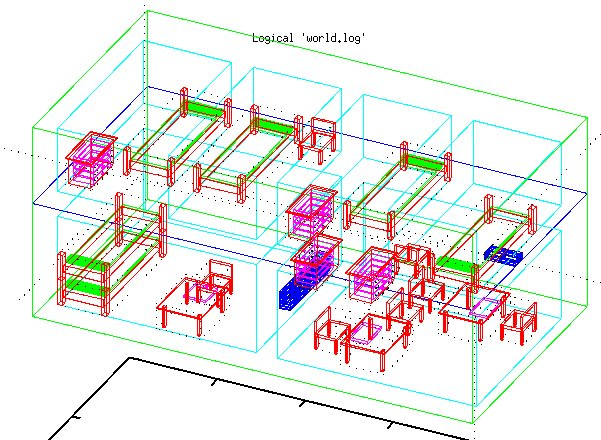
\includegraphics[width=\linewidth]{\imagepath/dm_world_0.jpeg}}
\end{center}
\caption{The  Devil's house  geometry  model. Rooms  display in  cyan,
  furniture  objects  (bed,  table,  chair\dots)  in  red,  drawer  in
  magenta, mailboxes in blue.}\label{fig:mapping:0}
\end{figure}

\begin{figure}[h]
\begin{center}
\scalebox{1.0}{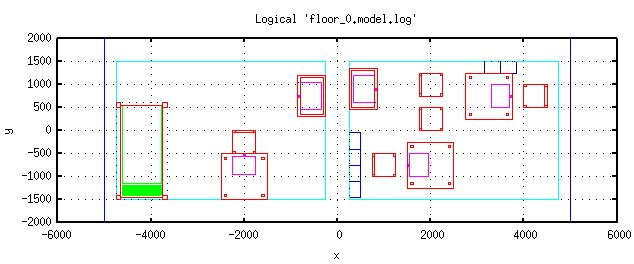
\includegraphics[width=\linewidth]{\imagepath/dm_floor_0.jpeg}}
\end{center}
\caption{Top   view    of   the   ground   floor    of   the   Devil's
  house.}\label{fig:mapping:1}
\end{figure}

\begin{figure}[h]
\begin{center}
\scalebox{1.0}{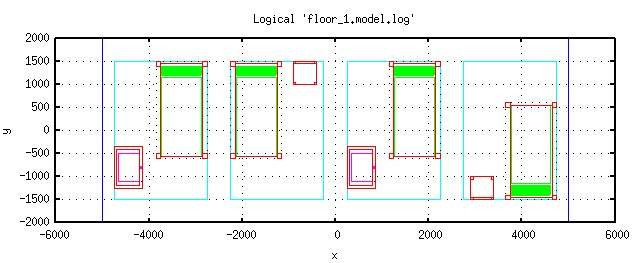
\includegraphics[width=\linewidth]{\imagepath/dm_floor_1.jpeg}}
\end{center}
\caption{Top   view    of   the    first   floor   of    the   Devil's
  house.}\label{fig:mapping:2}
\end{figure}
\clearpage
\subsubsection{Syntax}

\begin{sample}
\VerbatimInput[frame=single,
numbers=left,
numbersep=2pt,
firstline=3,
lastline=54,
fontsize=\footnotesize,
showspaces=false]{\codingpath/domestic_categories.lis}
\caption{The   geometry  categories   in  the   \textit{Devil's  house
    world}. Note  that the categories  are introduced from the  top of
  the hierarchy to the final leaves.}
\label{sample:mapping:0}
\end{sample}

There are 2 rooms on the ground floor (figure \ref{fig:mapping:1}) and
4 rooms  on the first  floor (figure \ref{fig:mapping:2}).   All rooms
contain   some  furnitures  like   beds,  chairs,   cupboards,  table,
mailboxes. These objects can be automatically associated to GIDs
through a geometry \emph{mapping} algorithm.  The
list  of  categories   is  defined  in  the  file   shown  in  sample
\ref{sample:mapping:0}.

The  geometry configuration  corresponding file  is shown  in appendix
\ref{app:mapping:0}.  Each  section related  to a geometry  model with
some daughter volumes to be  identified with a GID is \emph{decorated}
with    \emph{mapping}   directives.    For    example   the    sample
\ref{sample:mapping:1}  illustrates how  one attributes  a GID  to the
unique  house of  this  world :  this  GID belongs  to the  \TT{house}
category and its one-level address  is simply made of the house number
(labelled \TT{house\_number} in the sample file \ref{sample:mapping:0}) which
is arbitrarily chosen to \texttt{666}.


\begin{sample}
\VerbatimInput[frame=single,
numbers=left,
numbersep=2pt,
firstline=638,
lastline=657,
fontsize=\footnotesize,
showspaces=false]{\codingpath/domestic_models.geom}
\caption{The mapping directive  for the \emph{house} model placed in
  the \emph{world} model.}
\label{sample:mapping:1}
\end{sample}

 Another    similar     example    is    shown     on    the    sample
 \ref{sample:mapping:2}.   It  sets  the   mapping  directive   for  a
 \emph{floor} models.

 \begin{sample}
   \VerbatimInput[frame=single,
     numbers=left,
     numbersep=2pt,
     firstline=621,
     lastline=636,
     fontsize=\footnotesize,
     showspaces=false]{\codingpath/domestic_models.geom}
   \caption{The mapping directives  for the \emph{floor} volumes 
     contained in the  \emph{house} model.}
   \label{sample:mapping:2}
 \end{sample}

In  the case  of the  replicated  placement of  some similar  daughter
volumes,    another   syntax    is   used    as   shown    on   sample
\ref{sample:mapping:3}.  Here,  the  \TT{small\_mailbox}  model  being
composed of the replication of  2 columns of compartments, the mapping
directive  \TT{column+0}  specifies  that  the \TT{column}  number  is
incremented  automatically  from  the  initial value  \texttt{0}.  The
\TT{small\_mailbox\_column} model  uses a similar  syntax (\TT{row+0})
to  identify  the \texttt{row}  number  of  the  mail compartments  it
contains.

\begin{sample}
  \VerbatimInput[frame=single,
    numbers=left,
    numbersep=2pt,
    firstline=421,
    lastline=430,
    fontsize=\footnotesize,
    showspaces=false]{\codingpath/domestic_models.geom}
  \caption{The mapping directive  for the \emph{small mailbox column} volumes 
    contained in the  \emph{small mailbox} model.}
  \label{sample:mapping:3}
\end{sample}

Finally, another syntax  is used to number the  drawer associated to a
given  table (figure \ref{fig:mapping:3}). 

\begin{figure}[h]
  \begin{center}
    \scalebox{1.0}{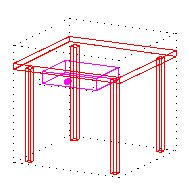
\includegraphics[width=0.3\linewidth]{\imagepath/dm_table_0.jpeg}}
    \scalebox{1.0}{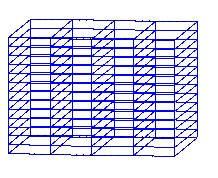
\includegraphics[width=0.3\linewidth]{\imagepath/dm_mailbox_0.jpeg}}
  \end{center}
  \caption{Left: the model of a table with its unique daughter drawer;
    right:  the  model  of  some  mailboxes that  corresponds  to  the
    replication  of  4  columns   each  of  13  vertically  replicated
    compartments.}\label{fig:mapping:3}
\end{figure}

This is shown on  sample \ref{sample:mapping:4}; it is here sufficient
to  specify the  only  category  to which  the  drawer is  associated,
because it \emph{inherits} the addresses path of its mother table.

\begin{sample}
  \VerbatimInput[frame=single,
    numbers=left,
    numbersep=2pt,
    firstline=239,
    lastline=258,
    fontsize=\footnotesize,
    showspaces=false]{\codingpath/domestic_models.geom}
  \caption{The mapping directive  for the \emph{small drawer} object 
    contained in the  \emph{table} model.} 
  \label{sample:mapping:4}
\end{sample}

\clearpage

\subsubsection{Automatic GIDs generation}

Once the  geometry configuration file  has been enriched  with mapping
directives,  it  is  possible  to  ask  a  \texttt{geomtooms::mapping}
algorithm to build the list of all (or part) of the GIDs corresponding
to   the    objects   of    the   hierarchy.   


\begin{program}[h]
\VerbatimInput[frame=single,
numbers=left,
numbersep=2pt,
firstline=6,
lastline=58,
fontsize=\footnotesize,
showspaces=false]{\codingpath/gmanager.cxx}
\caption{A program with embedded \emph{geometry mapping} (part 1/2).}
\label{program:mapping:1}
\end{program}

\begin{program}[h]
\VerbatimInput[frame=single,
numbers=left,
numbersep=2pt,
firstline=60,
fontsize=\footnotesize,
showspaces=false]{\codingpath/gmanager.cxx}
\caption{A program with embedded \emph{geometry mapping} (part 2/2).}
\label{program:mapping:2}
\end{program}

The   sample  program  \ref{program:mapping:1}-\ref{program:mapping:2}
illustrates the combined use of:
\begin{itemize}

\item  a \emph{geometry  factory}  which builds  the virtual  geometry
  setup from  a geometry description file; the  list of \emph{geometry
    models}   handled   by   the    factory   is   given   in   sample
  \ref{sample:mapping:gm:0}

\begin{sample}[h]
\VerbatimInput[frame=single,
numbers=left,
numbersep=2pt,
firstline=2,
lastline=35,
fontsize=\footnotesize,
showspaces=false]{\codingpath/gmanager.out}
\caption{The list of \emph{geometry  models} handled by the factory in
  program \ref{program:mapping:1}.}
\label{sample:mapping:gm:0}
\end{sample}

\item a \emph{GID manager} which handles a list of geometry categories
  loaded from a category description file,

\item a  \emph{mapping} algorithm  which reads the  mapping directives
  associated to  the models and create a  dictionary of \emph{geometry
    informations} associated to all geometry objects requested by some
  criteria; here we choose to :
  \begin{itemize}
    \item not limit  the generation of the dictionary  to some maximum
      depth in the hierarchy:
      \begin{CppVerbatim}
the_mapping.set_max_depth (geomtools::mapping::NO_MAX_DEPTH);
      \end{CppVerbatim}
    \item  not generate  the entries  that correspond  to  the objects
      identified as mail  compartments (the \TT{mailrow} category) and
      columns of mail compartments (the \TT{mailcolumn} category) :
     \begin{CppVerbatim}
the_mapping.add_excluded ("mailrow");
the_mapping.add_excluded ("mailcolumn");
      \end{CppVerbatim}

     The  list  of GIDs  associated  to  the generated  \emph{geometry
       information}      entries      is      given     id      sample
     \ref{sample:mapping:gm:1}.

     \begin{sample}[h]
       \VerbatimInput[frame=single,
         numbers=left,
         numbersep=2pt,
         firstline=39,
         lastline=86,
         fontsize=\footnotesize,
         showspaces=false]{\codingpath/gmanager.out}
       \caption{The  list of  \emph{geometry  information} entries  in
         program  \ref{program:mapping:2}. Here the  GID corresponding
         to the  \TT{mailrow} (type=42) and  \TT{mailcolumn} (type=41)
         have not been generated because of a the use of 
         some special mapping  exclusion directives (see text).}
       \label{sample:mapping:gm:1}
     \end{sample}

  \end{itemize}
 

\item a \emph{Gnuplot drawer} which display a 2D or 3D view of the virtual
  geometry setup.

\end{itemize}
\clearpage


%% end of mapping.tex
